\chapter{Test szybkości systemu}
\label{chap:test-szybkosci}
W tym rozdziale opisano badanie sprawdzające ile czasu zajmuje systemowi wykonanie wszystkich zadań koniecznych do wyświetlenia przetworzonej klatki obrazu. Porównano w nim m.in. wpływ rozdzielczości kamery. Pomiary zrealizowano dla trzech różnych ustawień rozdzielczości tej samej kamery: 640x360px, 640x480px i 1280x720px.
Według informacji pobranych z kamery za pomocą biblioteki OpenCV, operuje ona w 30 klatkach na sekundę, co daje około 33.33 milisekund na pojedyńczą klatkę. Liczba klatek użytych do testu to pięć tysięcy dla każdej rodzielczości.
Test wykonano na komputerze wyposażonym w kartę graficzną \emph{NVIDIA GeForce GTX 1650} i procesor \emph{Intel Core i5-8300H 2.30GHz}.

Poprzez czas potrzebny do wyświetlenia klatki rozumie się szereg czynności. Jest to proces rozpoczynający się od pobrania klatki z kamery, następnie detekcji obiektów oraz przetworzenia klatki w celu oznaczenia wykrytych obiektów, a kończący się poprzez wyświetlenie przetworzonej klatki obrazu przez graficzny interfejs użytkownika. 

W teście zmierzono całkowity czas do wyświetlenia wszystkich klatek oraz czas potrzebny do wyświetlenia pojedyńczej klatki (pięć tysięcy pomiarów na każdą rozdzielczość). Czas zmierzono poprzez pobranie w dwóch punktach -- początkowym i końcowym -- kodu źródłowego aktualnego czasu w systemie operacyjnym i obliczeniu różnicy jaka wystąpiła między tymi punktami. 

Dla pomiaru czasu całkowitego punkt początowy umiesczono po wyświetleniu przez GUI pierwszej klatki (klatka zerowa --- niewliczona do pomiaru). Punkt końcowy zmierzono po wyświetleniu ostatniej klatki.
Dla pojedyńczego pomiaru punkt początkowy jest taki sam dla pierwszej uwzględnionej klatki. Punkt końcowy jest ustawiany po wyświetleniu następnej klatki, w tym momencie też punkt końcowy staje się punktem początkowym dla pomiaru dla kolejnej klatki.
Pomiary czasu całkowitego dla zbadanych rozdzielczości kamery przedstawiono w tabeli \ref{tab:czas-calkowity-5000klatek}. Tabela uwzględnia zmierzony czas całkowity oraz obliczony na jej podstawie średni czas na klatkę oraz liczbę klatek na sekundę (FPS). Średni czas na klatkę obliczono poprzez podzielienie liczby klatek (5000) przez czas całkowity, natomiast FPS poprzez podzielenie liczby klatek przez czas całkowity.  
\begin{table}[H]
\centering
\caption{Pomiar czasu potrzebnego do wyświetlenia 5000 klatek.}
\begin{tabular}{|c|c|c|c|}
\hline
Rozdzielczość & Średni czas na klatke {[}ms{]} & Czas całkowity {[}s{]} & FPS   \\ \hline
640x360px     & 33.34                          & 166.69                 & 30    \\ \hline
640x480px     & 33.48                          & 167.42                 & 29.87 \\ \hline
1280x720px    & 33.58                          & 167.89                 & 29.78 \\ \hline
\end{tabular}
\label{tab:czas-calkowity-5000klatek}
\end{table}

Pomiary czasu całkowitego pokazały brak wpływu rozdzielczości kamery na szybkość systemu. Przyczynę takiego zachowania można upatrywać w optymalizacji YOLOv8, bowiem model ten przed rozpoczęciem detekcji skaluje obraz wejściowy do stałego rozmiaru -- do domyślnego rozmiaru lub ustawionego przez programistę parametrem inferencji \emph{imgsz} -- i wykonuje detekcję na przeskalowanym obrazie. Z racji braku opisu w dokumentacji modelu \cite{yolo_docs}, potwierdzenie istnienia tego mechanizmu opisano jako odpowiedź do pytania zadanego na forum, które jest umieszczone razem z repozytorium kodu modelu \cite{github_imgsz}.

Interesującą obserwacją jest również osiągnięcie liczby klatek na sekundę równej FPS kamery. Powodem może być np. przyśpieszone dostarczanie klatek przez samą kamerę.

Pomiary czasu całkowitego nie obrazują jednak potencjalnych odchyleń od średniej. Dlatego też postanowiono zilustrować pojedyńcze pomiary. Wykresy punktowe na rysnkach \ref{fig:czas-punktowy1}, \ref{fig:czas-punktowy2} i \ref{fig:czas-punktowy3} przedstawiają te pomiary i zestawiają je wraz z odpowiadającym średnim czasem z tabeli \ref{tab:liczba-klatek}. Aby sprawdzić różnicę w odchyleniach pomiędzy rozdzielczościami, dane z powyżej wspomnianych wykresów scalono na wykresie na ryskunku \ref{fig:czas-punktowy-all}.  


\begin{figure}[H]
    \centering
    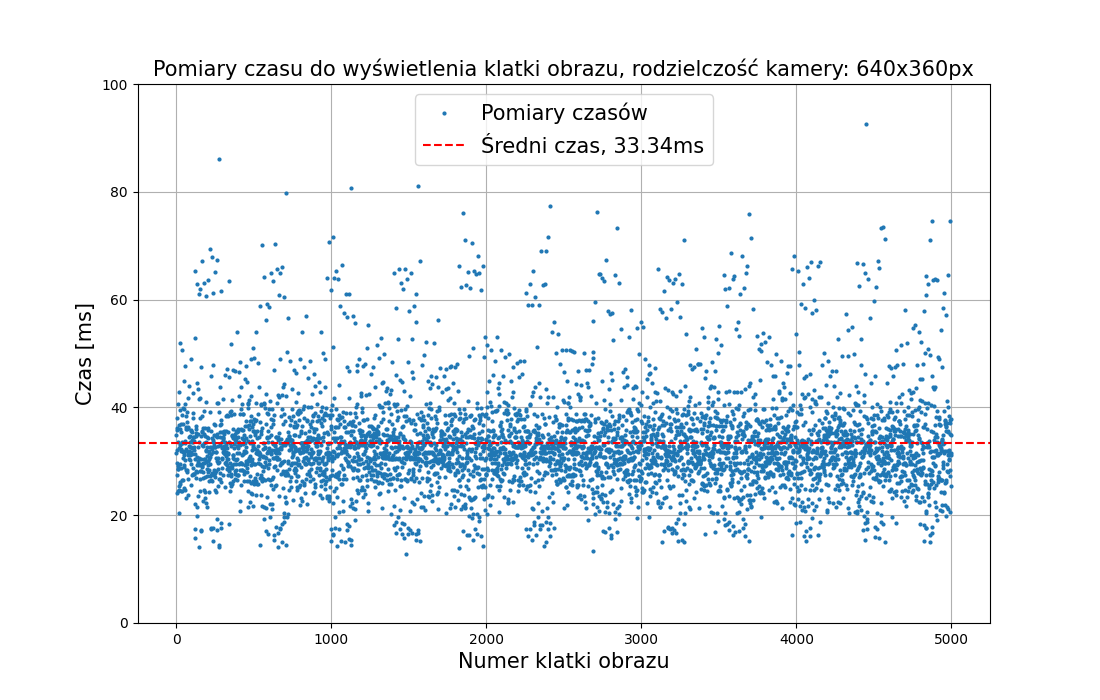
\includegraphics[width=\linewidth]{r_test_szybkosci/punkty/1.png}
    \caption{Wykres punktowy dla rodzielczości 640x360px przedstawiający pomiary czasu do wyświetlenia obrazu dla każdej klatki.}
    \label{fig:czas-punktowy1}    
\end{figure}

\begin{figure}[H]
    \centering
    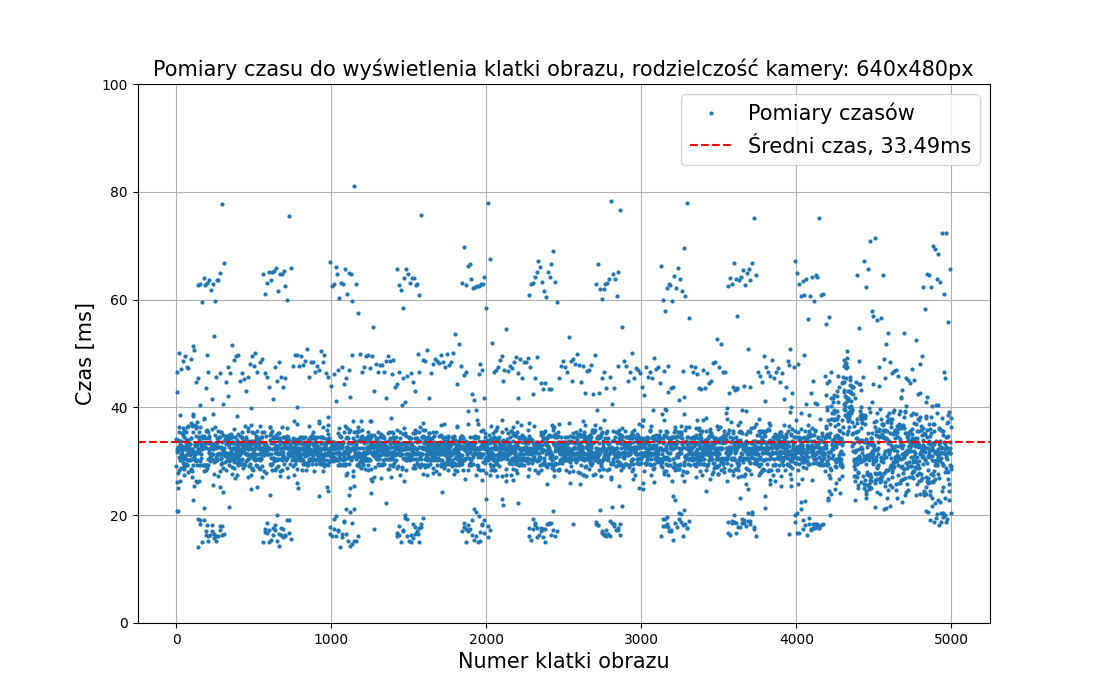
\includegraphics[width=\linewidth]{r_test_szybkosci/punkty/2.png}
    \caption{Wykres punktowy dla rodzielczości 640x480px przedstawiający pomiary czasu do wyświetlenia obrazu dla każdej klatki.}
    \label{fig:czas-punktowy2}    
\end{figure}

\begin{figure}[H]
    \centering
    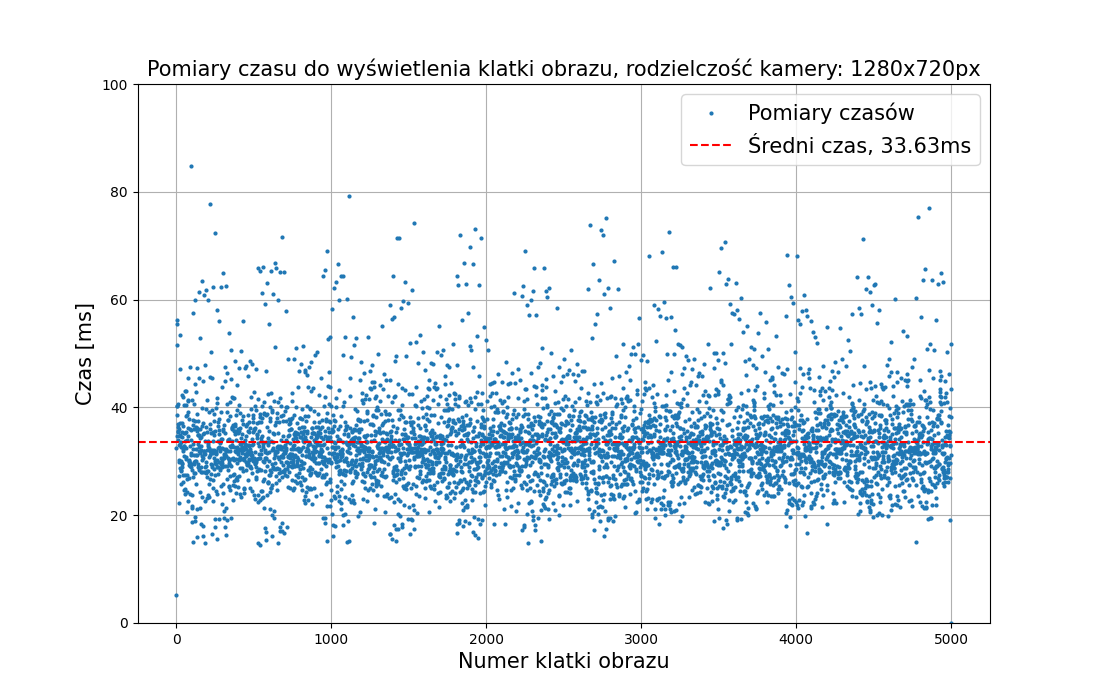
\includegraphics[width=\linewidth]{r_test_szybkosci/punkty/3.png}
    \caption{Wykres punktowy dla rodzielczości 1280x720px przedstawiający pomiary czasu do wyświetlenia obrazu dla każdej klatki.}
    \label{fig:czas-punktowy3}    
\end{figure}

\begin{figure}[H]
    \centering
    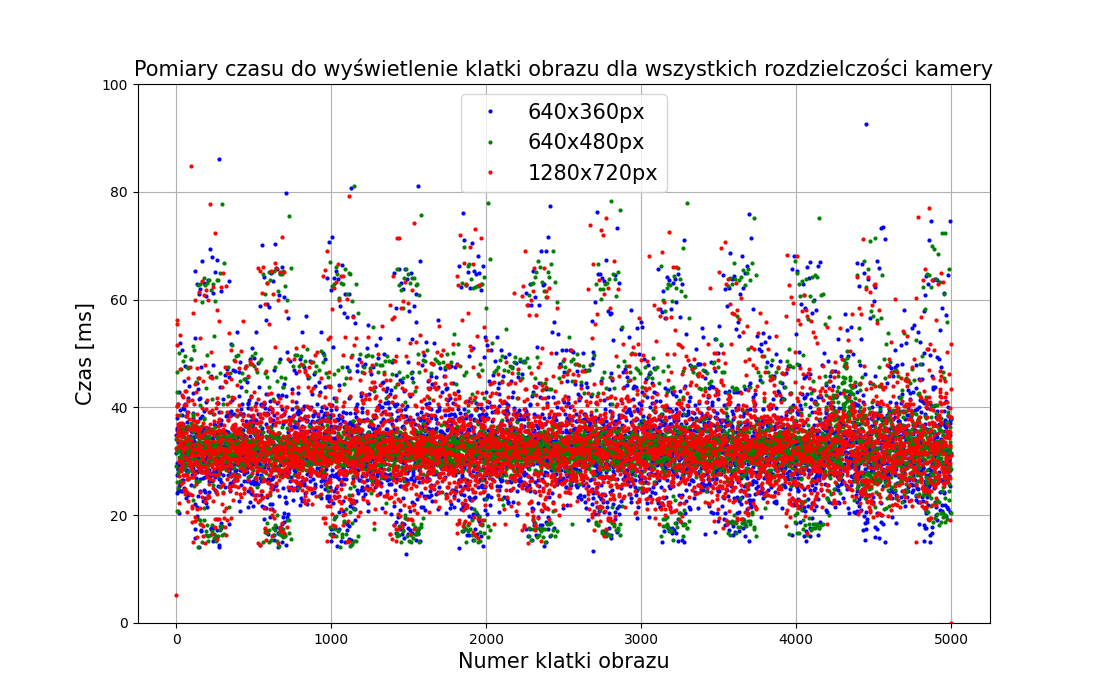
\includegraphics[width=\linewidth]{r_test_szybkosci/punkty/all.png}
    \caption{Wykres punktowy dla wszystich rozdzielczości przedstawiający pomiary czasu do wyświetlenia obrazu dla każdej klatki.}
    \label{fig:czas-punktowy-all}    
\end{figure}

Dla wyników dla każdej rozdzielczości można zaobserwować zagęsczenie punktów przy średniej wartości. 
Zagęsczenie pomiędzy rozdzielczościami można ocenić na podobne, chociaż na korzyść wyróżnia się rozdzielczośc 640x480px. Może być to spowodowane tym, że jest to ustawienie najbliżej odpowiadające użytemu, domyślnemu rozmiarowi obrazu poddanemu detekcji w YOLOv8n, które wynosi 640x640px. Wpływ mogły mieć również czynniki zewnętrzene takie jak mniejsze zajęcia procesora przez inne programy działające w komputerze.  

Zagęszczenie pokazuje pewien stopień powtarzalności. Mimo to na tym etapie testów system nie można uznać za powtarzalny. Liczba przetestowanych klatek nie pozwala wizualnie ocenić charakterystyki odchyleń od średniej. W celu dalszych testów możnaby możnaby parokrotnie zbadać mniejszą liczbe klatek i sprawdzić czy odchylenia mają naturę całkowicie losową albo czy występuje pewna zależność np. wystąpienie pewnego podzbioru, dla którego odchylenia najpierw rosną, a później maleją. Wykonanie takiego badania nie jest natomiast w pełni konieczne. Priorytetem systemu jest alarmowanie użytkownika z możliwie jak najmniejszym opóźniem, co eliminuje konieczność utrzymania stałego czasu wykonania. Biorąc to pod uwagę badaniu poddanoby tylko odchylenia większe od średniej. 

Sam fakt wystąpienia odchyleń nie definiuje jak bardzo opóźnione są alarmy wysyłane przez system. Wykresy pokazały, że nawet w sytuacji wystąpienia odchylenia, wyniki dla kolejnych klatek dalej są w większości zagęszczone w okolicy średniej i ponadto nie wystąpiła uznana za znaczącą zmiana w stopniu zagęsczenia. Dodatkowo wykres na ryskunku \ref{fig:czas-punktowy-all} pokazał również, iż zakres odchyleń można zaklasyfikować do tego samego zbioru dla wszystkich rozdzielczości.   
Podczas wykorzystania systemu jako użytkownik jakościowo stwierdzono, iż opóźnienia w alarmowaniu są niezauważalne. 

Podsumowując, dla wykorzystanego wyposażenia sprzętowego, wykazano niezależność wyników od ustawionej rozdzielczości kamery. Ponadto stwierdzono, iż opóźnienia systemu z wynikających odchyleń od średniej nie wpływają na komfort użytkowania.

